
\chapter{直觉}
\label{chap:intuition}

\section{概率问题}
\label{sec:probability-issues}

\begin{example}[被针对的先手玩家]
  这是一个充满陷阱的游戏,因为无论如何后选者都办法使自己的获胜机会大于先选者。

  具体游戏规则如下。抛三次硬币,看猜哪面朝上,其组合共$2^3=8$种。两个玩家,玩家1先选其中一组组合,然后玩家2再选一组不同的组合。选定后,找人连续不停地抛硬币,直到某个玩家选定的组合出现为止,谁选的组合先出现谁获得胜利。

  对于这个游戏,后选的玩家是否有策略让自己获胜的概率高于先选玩家?
\end{example}
\begin{proof}[提示]
  因为每种组合出现的概率都是一样,所以如果有人直觉地认为不管如何选择,先选和后选获胜的概率应该是一样的,这一点都不奇怪。但必须请有这种直觉的人注意,这种直觉遗留了某些东西。实际上,后选玩家如果针对先选玩家的选择做出合适的策略的话,后选玩家获胜的概率是可以提高的。

  比如,如果先选玩家选择“反反反”这种组合,那么后选玩家可以选择“正反反”。那么除非头三次抛硬币就出现了“反反反”,否则先选玩家再也没机会取胜了,因为在出现“反反反”之时,一定会有一个“正”在前面,即有“正反反反”的模式,后选玩家的“正反反”早已在“反反反”之前获胜了。后选玩家获胜的概率是7/8。

  后选者的一个策略,是
  \begin{quotation}
    我能利用你获胜的条件,而你不能利用我获胜的条件。换言之,你获胜的状态对我有帮助,而我获胜的状态对你没帮助。
  \end{quotation}

  先引入记号,记$\bar a$为与$a$相反的面,即若$a$为正,则$\bar a$为反;若$a$为反,则$\bar a$为正。

  一般来说,若先选的为$abc$,则后选有两个选择$xab$,其中$x$可能为“正”也可能为“反”,换而言之,$x$可能为$c$也可能为$\bar c$。分别考虑:
  \begin{enumerate}
  \item 什么时候选$cab$,为了使$cab$是好的策略,必须不能让先选者利用$cab$的前两个$ca$及更前面的$x$来凑成$abc$,即$xca\ne abc$,从而只要$ca\ne bc$即可,即$c\ne b$或者$c\ne a$;
  \item 什么时候选$\bar cab$,同样只要$\bar ca\ne bc$即可,即$\bar c\ne b$或者$c\ne a$,等价于$c=b$或者$c\ne a$。
  \end{enumerate}

  综上,若$c=b$,后选者可选$\bar cab$;若$c\ne b$,后选者可选$cab$。这是其中一种针对选择方法。若用1表示正,0表示反,则此种针对选法如表~\ref{tab:3-coins-trap-game}所示:
  \begin{table}[htbp]
    \centering
    \begin{tabular}{cccc}
      \toprule
      序号 & 先选者的选择 & 后选者的针对选择 & 后选者获胜的概率 \\\midrule
      1 & 000 & 100 & 7/8\\
      2 & 001 & 100 & 3/4\\
      3 & 010 & 001 &\\
      4 & 011 & 001 &\\
      5 & 100 & 110 &\\
      6 & 101 & 110 &\\
      7 & 110 & 011 &\\
      8 & 111 & 011 &\\
      \bottomrule
    \end{tabular}
    \caption{三次硬币组合的后选针对选法}
    \label{tab:3-coins-trap-game}
  \end{table}

  由表格可以看出,序号1和8是对称的,2和7是对称的,3和6是对称的,4和5是对称的,即$n$和$9-n$是对称的。实际上,只要把0看作1,把1看作0,即记号反过来写,用0表示“正”,用1表示“反”,则两种情况可以共用同一种分析方法,所以两种对称情况后选者获胜的概率是一致的。下面分析前4种情况后选者的获胜概率。

  首先,容易得到下面的结论:
  \begin{quotation}
    若某次抛硬币结果后,两人都没有获胜,则只有最后的3次的结果对后续有影响。
  \end{quotation}
  如某次抛完硬币后的所有正反面结果为001101,且两人都未获胜,则后续只需保留末尾的101继续考虑即可。
  
  \begin{enumerate}
  \item[\underline{000}] 前面已经分析了,前3次抛硬币的结果,只有000能使先选者获胜,其余7种都使后选者获胜,所以后选者获胜的概率为7/8。
  \item[\underline{001}] 画出头3枚硬币的8种初始状态的路径图,如图~\ref{fig:path-of-001},其中阴影部分节点代表了头三次抛硬币结果的8种状态,1W表示先选者胜利,2W表示后选者胜利。可以看出,硬币无限抛下去的话,只有头3枚硬币是000和001的状态先选玩家获胜,其余的6种初始状态都是后选玩家获胜,从而其概率是3/4。
  \item[\underline{其余}] 请画出状态路径图计算后选者策略的获胜概率。
  \end{enumerate}
  \begin{figure}[htbp]
    \centering
    \begin{tikzpicture}[scale=2.0]
      \begin{scope}[shift={(0,0)}]
        \node[draw,circle,fill=red!20](O) at(0,0) {000};
        \node[draw,circle](O2) at(1,0) {0001};
        \node[draw,circle,fill=red!20](O4) at(2,0) {001};
        \node[draw,circle](O1) at(1,1) {0000};
        \node(W) at(3,0) {1W};
        \draw[->](O)edge[bend left=20](O1);
        \draw[->](O1)edge[bend left=20](O);
        \draw[->](O)--(O2);
        \draw[->](O2)--(O4);
        \draw[->](O4)--(W);
      \end{scope}
    % \end{tikzpicture}
    % 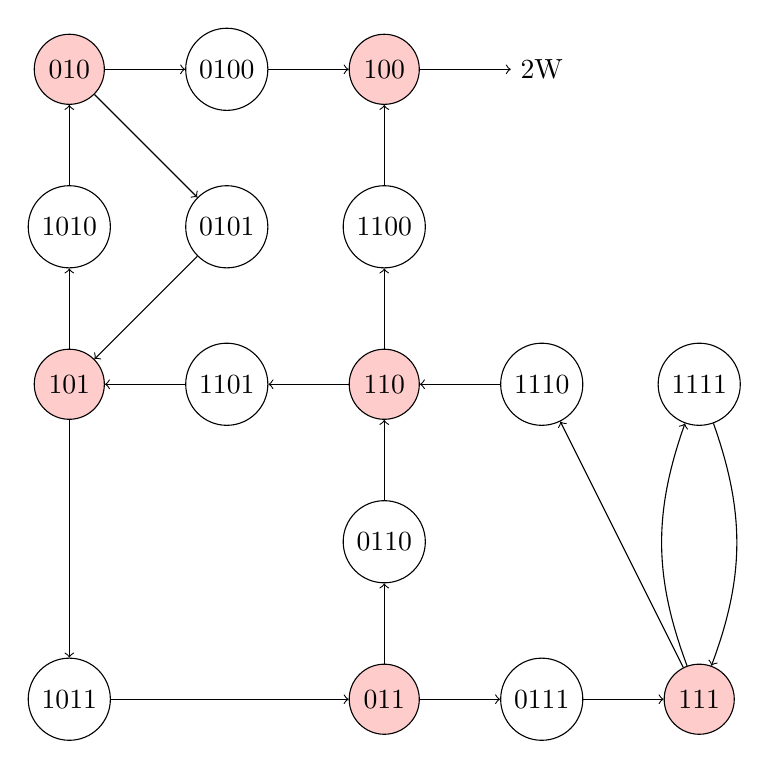
\begin{tikzpicture}[scale=2]
      \begin{scope}[shift={(0,-5)}]
        \node[draw,circle,fill=red!20](N010) at(0,4) {010};
        \node[draw,circle](N0100) at(1,4) {0100};
        \node[draw,circle,fill=red!20](N100)  at(2,4) {100};
        \node(W)     at(3,4) {2W};
        \node[draw,circle](N1010) at(0,3) {1010};
        \node[draw,circle](N0101) at(1,3) {0101};
        \node[draw,circle](N1100) at(2,3) {1100};
        \node[draw,circle,fill=red!20](N101)  at(0,2) {101};
        \node[draw,circle](N1101) at(1,2) {1101};
        \node[draw,circle,fill=red!20](N110)  at(2,2) {110};
        \node[draw,circle](N1110) at(3,2) {1110};
        \node[draw,circle](N1111) at(4,2) {1111};
        \node[draw,circle](N0110) at(2,1) {0110};
        \node[draw,circle](N1011) at(0,0) {1011};
        \node[draw,circle,fill=red!20](N011)  at(2,0) {011};
        \node[draw,circle](N0111) at(3,0) {0111};
        \node[draw,circle,fill=red!20](N111)  at(4,0) {111};

        \foreach \x/\y in{N010/N0100, N0100/N100, N100/W,
          N010/N0101, N1010/N010, N101/N1010,N1100/N100,N0101/N101,
          N1101/N101,N110/N1101,N110/N1100,N1110/N110,N0110/N110,
          N101/N1011,N1011/N011,N011/N0110,N011/N0111,N0111/N111,
          N111/N1110%
        }{
          \draw[->](\x)--(\y);
        }
        \draw[->](N111)edge[bend left=20](N1111);
        \draw[->](N1111)edge[bend left=20](N111);
      \end{scope}
    \end{tikzpicture}
    \caption{先选者选择001时的状态路径}
    \label{fig:path-of-001}
  \end{figure}

  表格~\ref{tab:3-coins-trap-game}只是使后选者获胜概率高于先选者的一种充分方法,那么是否是必要方法呢?若有兴趣,请自行思考。
\end{proof}

\begin{example}[三门问题,蒙提霍尔问题,Monty Hall problem]
  在美国的一个Monty Hall主持的电视节目Let's Make a Deal上,会邀请参与者玩一个游戏:参与者会看见三扇关闭的门,其中一扇后面有一辆汽车,其余两辆后面各有一只山羊。参与者可以选择其中一扇门,从而赢得此门背后对应的汽车或山羊。为了制造气氛,在参与者选中一扇门后但未开启时,主持人会开启剩余两扇门的一扇,露出其后面的山羊,然后询问参与者是否要更换另一扇仍然关闭着的门。如果参与者为了使赢得汽车的概率最大化,他应该换还是不换?

  为了使问题更清晰不含糊,下面是额外的前提假设。
  \begin{enumerate}
  \item 汽车事前是等可能地被放置于三扇门的其中一扇后面;
  \item 参赛者在三扇门中挑选时并不知道任意一扇门后面是什麽;
  \item 主持人知道每扇门后面有什么;
  \item 如果参赛者挑了一扇有山羊的门,主持人必须开启另一扇有山羊的门;
  \item 如果参赛者挑了一扇有汽车的门,主持人等可能地开启另外两扇有山羊的门中的其中一扇。
  \end{enumerate}
\end{example}
\begin{proof}[说明]
  一种比较直观的看法,是任意一扇门背后是汽车的概率都是1/3,主持人打开一扇有山羊的门后,并不影响另一扇门背后是汽车的概率,因为背后摆放的物品早已确定。

  还有一种也比较直观的看法,是当主持人打开一扇有山羊的门后,剩余两扇门背后是汽车的概率都是1/2,所以换与不换都是一样的。

  然而事实是这样吗?再看下面的观点。把参与者初始选择的门编号为1,其余两扇门分别编号为2和3。则可能的初始状态如表~\ref{tab:states-of-3-gates}。

  \begin{table}
    \caption{三门问题状态列表}
    \label{tab:states-of-3-gates}
    \centering
    \begin{tabular}{c|c|cc||c|c}
      \hlineB{2}
      \multirow{2}{1.5cm}{初始状态序号} & \multicolumn{3}{c||}{门}  &\multicolumn{2}{c}{主持人开启一扇门后}\\
      \cline{2-6}                   & 1    &  2   &  3    & 1    & 另一扇关闭的门 \\\hline
      1                             & 汽车 & 山羊 & 山羊  & 汽车 & 山羊\\
      2                             & 山羊 & 汽车 & 山羊  & 山羊 & 汽车\\
      3                             & 山羊 & 山羊 & 汽车  & 山羊 & 汽车\\
      \hlineB{2}
    \end{tabular}
  \end{table}

  对于不更换选择的策略,只有初始状态1可以赢得汽车,概率为1/3。而对于更换选择的策略,初始状态2和3都可以赢得汽车,概率为2/3。所以更好的策略是更换选择。

  还有一种看法是,当主持人开启一扇门后,更换选择的话,相当于二选一,能赢得汽车的概率为1/2,而不更换的话,概率不会改变,还是初始的1/3。所以更好的策略还是更换选择。

  2008年的美国电影《决胜21点》(英文就叫21)也有这个故事。
\end{proof}


\begin{example}[贝特朗悖论,Bertrand paradox]
  在单位圆内的弦中随机选一条,其长度超过圆内接三角形边长的概率是多少?
\end{example}
贝特朗提出这个问题时给出了三个都是正确的但结论不一样的解法。三种方法的区别在于选取弦的方法。

\begin{enumerate}
\item 通过两个端点确定弦。假设圆内弦的端点在圆周上是均分布的,可得概率为$1/3$。在圆周任意选取两点,相当于固定一点,在圆周上任意选取另外一点。在固定点上作为一个顶点作圆内接正三角形。显然当且仅当另一端落中图中阴影部分的圆弧上时此两点组成的弦超过三角形的边长。即概率为1/3。
\item 通过到圆心的距离确定弦。假设圆内弦到圆心的距离是均匀分布的,可得概率为$1/2$。不妨只考虑某特定方向的弦,且只考虑半圆,则如图2,只有图中阴影部分的弦长度超过三角形边长,其面积为半圆的一半。
\item 通过弦的中点确定弦。假设圆内弦的中点在圆内是均匀分布的,可得概率为$1/4$。如图3,只有弦的中点在阴影圆内时弦的长度才能超过三角形边长,其面积为单位圆面积的$1/4$。
\end{enumerate}

\begin{figure}[htbp]\centering
  \begin{tikzpicture}[scale=.9]
    \begin{scope}[shift={(0,0)}]
      \coordinate (A) at ( 90:2);
      \coordinate (B) at (210:2);
      \coordinate (C) at (330:2);
      \fill[red!20](A)--(B)arc(210:330:2)--(A);
      \draw[very thick](0,0)circle(2) (A)--(B)--(C)--(A);
      \coordinate(A1) at (180:2);
      \coordinate(A2) at (250:2);
      \coordinate(A3) at (280:2);
      \coordinate(A4) at (30:2);
      \draw[help lines, dashed](A)--(A1) (A)--(A2) (A)--(A3) (A)--(A4);
      \node[below] at(0,-2.2){端点在圆周上均匀分布};
      \tkzDrawPoints(A,A1,A2,A3,A4)
    \end{scope}
    \begin{scope}[shift={(5,0)}]
      \coordinate (A) at ( 90:2);
      \coordinate (B) at (210:2);
      \coordinate (C) at (330:2);
      % \fill[red!20](A)--(B)arc(210:330:2)--(A);
      \fill[red!20](2,0)--(-2,0)arc(180:210:2)--(C)arc(330:360:2);
      \draw[very thick](0,0)circle(2) (A)--(B)--(C)--(A);
      \draw(0,0)--(0,-2) (2,0)--(-2,0);
      % \tkzDrawPoint(A)
      \coordinate(A1) at (190:2); \coordinate(B1) at (350:2);
      \coordinate(A2) at (200:2); \coordinate(B2) at (340:2);
      \coordinate(A3) at (230:2); \coordinate(B3) at (310:2);
      \coordinate(A4) at (250:2); \coordinate(B4) at (290:2);
      \draw[help lines, dashed] (A1)--(B1) (A2)--(B2) (A3)--(B3) (A4)--(B4);
      \node[below] at(0,-2.2){到圆心的距离均匀分布};
      \coordinate(O) at (0,0);
      \coordinate (P1) at ($(A1)!(O)!(B1)$);
      \coordinate (P2) at ($(A2)!(O)!(B2)$);
      \coordinate (P3) at ($(A3)!(O)!(B3)$);
      \coordinate (P4) at ($(A4)!(O)!(B4)$);
      \tkzDrawPoints(P1,P2,P3,P4);
    \end{scope}
    \begin{scope}[shift={(10,0)}]
      \coordinate (A) at ( 90:2);
      \coordinate (B) at (210:2);
      \coordinate (C) at (330:2);
      %\fill[red!20](A)--(B)arc(210:330:2)--(A);
      \draw[very thick](0,0)circle(2) (A)--(B)--(C)--(A);
      \draw(0,0)[fill=red!20]circle(1);
      %\tkzDrawPoint(A)
      \node[below] at(0,-2.2){中点在圆内均匀分布};
      \coordinate(A1) at (110:2); \coordinate(B1) at (220:2); \coordinate(C1) at($.5*(A1)+.5*(B1)$);
      \coordinate(A2) at (135:2); \coordinate(B2) at (300:2); \coordinate(C2) at($.5*(A2)+.5*(B2)$);
      \coordinate(A3) at (260:2); \coordinate(B3) at ( 70:2); \coordinate(C3) at($.5*(A3)+.5*(B3)$);
      \coordinate(A4) at (150:2); \coordinate(B4) at ( 30:2); \coordinate(C4) at($.5*(A4)+.5*(B4)$);
      \coordinate(A5) at ( 85:2); \coordinate(B5) at (350:2); \coordinate(C5) at($.5*(A5)+.5*(B5)$);
      \draw[help lines, dashed] (A1)--(B1) (A2)--(B2) (A3)--(B3) (A4)--(B4) (A5)--(B5);
      \tkzDrawPoints(C1,C2,C3,C4,C5);
    \end{scope}
  \end{tikzpicture}
  \caption{贝特朗问题的三种假设}
  \label{fig: Bertrand-assumptions}
\end{figure}

造成同一个问题有不同的答案,其根源在于三种解法使用了不同的假设,从而导致了样本空间不一致。三种解法的样本空间分别是:
\begin{enumerate}
\item 圆周上的点组成的样本空间;
\item 半径上的点组成的样本空间;
\item 大圆内的点组成的样本空间。
\end{enumerate}

此悖论说明,在定义概率时要事先确定样本空间,不同的样本空间会导致不同的概率结果。